% @Author: Sol W Courtney
% @Date:   2018-03-19 01:09:29
% @Last Modified by:   Sol W. Courtney
% @Last Modified time: 2018-03-19 03:15:19
% Author 	: Sol W. Courtney
% Location 	: Columbia U Dept. of Astronomy & Astrophysics NYC, Ny
% Email 	: swc2124@Columbia.edu
% Date 		: October 2016
%% --------------------------------------------------------------------------
%% DOCUMENT CLASS
%% --------------------------------------------------------------------------
\documentclass[11pt,a4paper,fleqn,notitlepage,oneside]{article}

%% --------------------------------------------------------------------------
%% PACKAGES
%% --------------------------------------------------------------------------
\usepackage[utf8]{inputenc}
\usepackage{lmodern}% http://ctan.org/pkg/lm
\usepackage{indentfirst}
\usepackage{siunitx}
\usepackage{float}
\usepackage{booktabs}
\usepackage{longtable}
\usepackage[letterpaper, margin=1in]{geometry}
\usepackage{pgf}
\usepackage[margin=2.5cm]{caption}
\usepackage{graphicx}
\graphicspath{
	{/home/sol/Github/skysearcher/data/plots/}
	{/home/sol/Github/skysearcher/data/plots/}
	}

%% --------------------------------------------------------------------------
%% TITLE
%% --------------------------------------------------------------------------
\title{Defining WFIRST Survey Parameters: \\ Computational Methods}
\author{Sol W. Courtney, Kathryn V. Johnston \& Robyn E. Sanderson \\ Columbia University Dept. Astronomy and Astrophysics}
\date{\today}

%% --------------------------------------------------------------------------
%% BEGIN DOCUMENT
%% --------------------------------------------------------------------------
\begin{document}
\maketitle

%% --------------------------------------------------------------------------
%% ABSTRACT
%% --------------------------------------------------------------------------
\begin{abstract}
	This document summarizes a first look at the possible parameters of a WFIRST survey of stellar halos around the 100 most luminous galaxies within 10Mpc of us. 
	There are broadly three aims of such surveys: (i) to look at the global properties of the halos (e.g. radial profile and total content); (ii) to find structures that are signatures of recent accretion events in order to examine broad properties and variety in accretion histories (including luminosity functions, rates and orbits); (iii) to find features at widest possible separations for subsequent spectroscopic follow up in order to place potential constraints.
	For all of the above purposes, the halos should be observed to the greatest radial extent possible.
	The extent to which this is possible or interesting will depend on expected densities of the stellar halos as well as contamination by background galaxies at faint magnitudes.
	The study “observes" the Bullock/Johnston stellar halo models as a guide for expectations (could be subsequently replaced with other models - e.g. FIRE).
\end{abstract}

%% --------------------------------------------------------------------------
%% STEP-BY-STEP
%% --------------------------------------------------------------------------
\section{The 100 Brightest Targets} % (fold)
	\label{sec:the_100_brightest_targets}

	\subsection{Karachentsev's catalog NEARGALCAT} % (fold)
		\label{sub:karachentsev_s_catalog_neargalcat}
		The Karachentsev\cite{2013AJ....145..101K} updated nearby galaxy catalog represents the nearest 869 galaxies.
		We are interested in observing those galaxies which are at least as luminous as the MilkyWay and therefore roughly equivalent in mass.
		Our goal is to sensibly select $100$\ targets from Karachentsev's original $869$\ galaxies.
		These target galaxies will serve as the underling layout for our simulated survey.
		\begin{table}[H]\centering
			\begin{tabular}{||c|cccc||}%\toprule[1.5pt]
				\hline 
				Unit & min & mean & max & std \\
				\midrule[1.5pt]
				$Distance\ (Mpc)$ & 0.02 & 6.98 & 26.2 & 4.19 \\
				$Abs_{B}mag$ & -21.8 & -13.83 & 0.0 & 3.42 \\
			\hline
			%\bottomrule[1.5pt]
			\end{tabular}
		\caption{
			Here we see the stats of the Karachentsev\cite{2013AJ....145..101K} catalog without the MilkyWay.
			$868$\ galaxies included.
			}
		\label{tab:1}
		\end{table}
	% subsection karachentsev_s_catalog_neargalcat (end)

	\subsection{Our Targets} % (fold)
		\label{sub:our_targets}
		After sorting the list by distance we then select those galaxies which have an estimated distance of less than $10\ Mpc$.
		We then take the $100$\ most luminous of these targets as our $100$\ prospective targets.
		After selecting the targets, we calculate the minimum intrinsic brightness a star would need to be $M_{ab}Limit$\ in order to be perceptible at each target's estimated distance with the following.
		\[
		M_{ab}Limit = m^{filter}_{t_{exp}}limit - 5 * log_{10}(Distance*10^{6}\ Mpc/10pc)\ 
		\]
		\begin{table}[H]\centering
			\begin{tabular}{||c|cccccc||}%\toprule[1.5pt]
				\hline 
				$Filter$ & Z087 & Y106 & J129 & H158 & F184 & W149\\
				\midrule[1.5pt]
				$1000\ second\ (m^{filter}_{1000sec}limit) $ & 27.15 & 27.13 & 27.14 & 27.12 & 26.15 & 27.67\\
				$2000\ second\ (m^{filter}_{2000sec}limit) $ & 27.9 & 27.88 & 27.89 & 27.87 & 26.9 & 28.42\\
				$t_{exp}$\ for $\sigma_{read}=\sigma_{sky}\ (seconds)$ & 200 & 190 & 180 & 180 & 240 & 90\\
			\hline
			%\bottomrule[1.5pt]
			\end{tabular}
		\caption{
			Here we see the WFIRST filter $1000$\ and $2000$\ second exposure imaging depths for each filter and $t_{exp}$\ for $\sigma_{read}=\sigma_{sky}\ (seconds)$
			}
		\label{tab:2}
		\end{table}

		From here onward we have selected the WFIRST H158 filter which has apparent magnitude limit of $27.87$\ when $t_{exp}=2000\ seconds$.
		The following table shows the $100$\ selected targets stats including the $M_{ab}Limit$\ for the target's distance as calculated with filter H158 for both $t_{exp}=1000\ seconds$\ and $t_{exp}=2000\ seconds$.
		$M_{ab}Limit$\ represents the estimated minimum intrinsic brightness a star needs to be precipitable.

		\begin{table}[H]\centering
			\begin{tabular}{||c|cccc||}%\toprule[1.5pt]
				\hline 
				Unit & min & mean & max & std \\
				\midrule[1.5pt]
				$Distance\ (Mpc)$ & 0.82 & 4.54 & 7.2 & 1.5 \\
				$Abs_{B}mag$ & -21.3 & -17.39 & -15.1 & 1.64 \\
				$1000\ seconds\ M_{ab}Limit$ & -3.137 & -1.99 & 1.581 & 0.87 \\
				$2000\ seconds\ M_{ab}Limit$ & -1.414 & 0.26 & 3.304 & 0.87 \\
			\hline
			%\bottomrule[1.5pt]
			\end{tabular}
		\caption{
			Here we see the stats of our $100$\ most luminous target galaxies.
			$M_{ab}Limit$\ represents the minimum intrinsic brightness a star would need be if it is to be precipitable at the targets' estimated distance assuming filter H158 for both 1000 and 2000 second exposure times.
			}
		\label{tab:3}
		\end{table}
	% subsection our_targets (end)
% section the_100_brightest_targets (end)

\section{Time Constraints} % (fold)
	\label{sec:time_constraints}
	The total required time for a survey seems to depend on 4 main factors.
	Fist there is the number of intended targets $(100)$.
	Second there is the extent of each halo intended to be photographed $(radial\ seperation\ Kpc)$.
	Third there is the estimated distance $(Mpc)$\ to each target and therefore the number of full fields of view $(N_{FoV})$.
	Fourth is the intended exposure time $(t_{exp})$\ for each $FoV$.
	Additionally there is the $slew/settle\ time$\ and the required time for target to target positioning.

	Putting this all together we can see that if $t_{exp}=2000\ seconds$\ one could tile/mosaic each of the 100 targets to a radial extent of 100 Kpc $(200\ Kpc\ box)$\ in approximately 2055 hours.
	Additionally there will be about 100 to 150 hours of movement.
	For a 200 Kpc box $(100\ Kpc\ seperation)$\ around each target there are in total approximately 3700 full WFIRST FoVs.
	Roughly 1241 square degrees in total, just about 3\% of the sky.

	Bellow is figure 1 showing the total $(in\ blue)$\ and cumulative $(in\ red)$\ amounts of both area $(on\ top)$\ and time $(on\ bottom)$\ associated with exposing a 200 Kpc box $(100\ Kpc\ seperation)$\ around each of our 100 proposed targets.
	The x-axis of both plots represents the distance to target, ranging from 0 to 8 $Mpc$.

	\begin{figure}[H]
		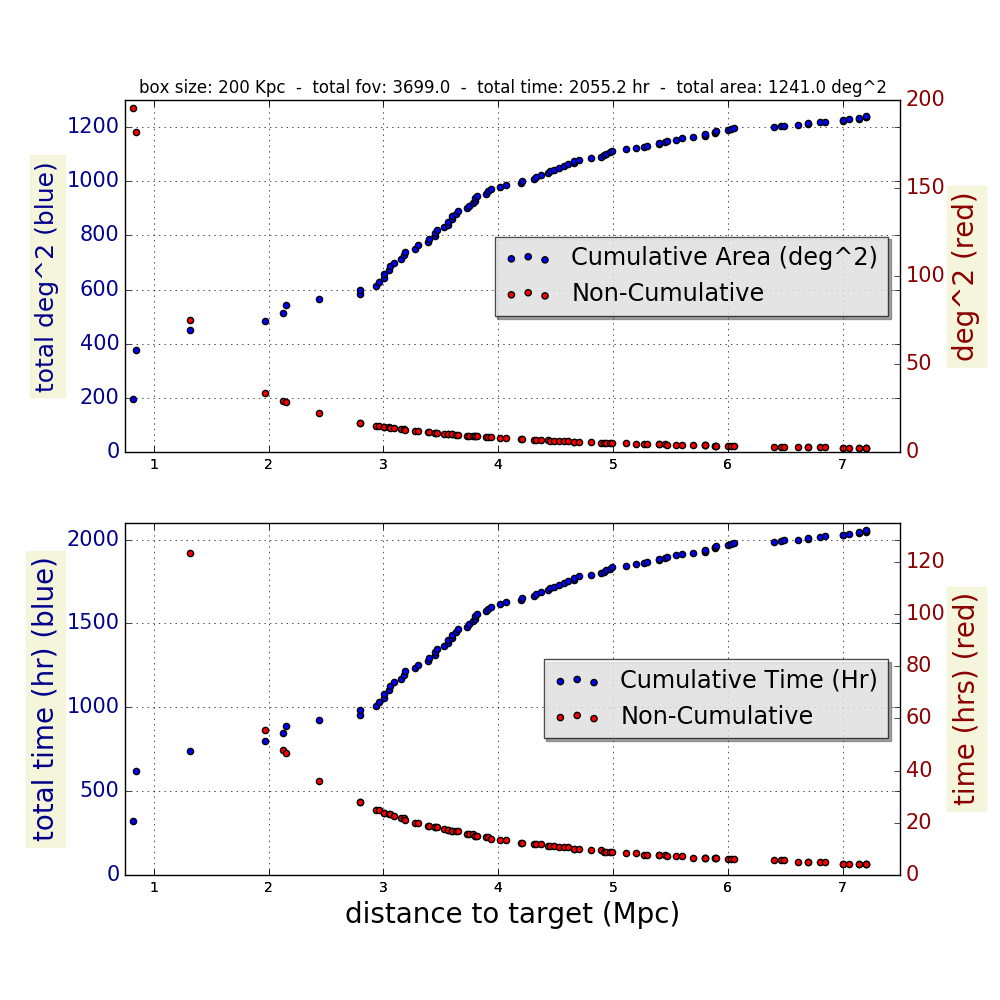
\includegraphics[width=17cm]{all_targets.png}
	\caption{
		The top plot shows the the individual $(in\ red)$\ and cumulative $(in\ blue)$\ area $(deg^{2})$ covered by all 100 proposed target galaxies each having a 200 Kpc box $(radial\ seperation\ of\ 100\ Kpc)$.
		The bottom plot shows both the number of hours required for each target $(in\ red)$\ and the associated cumulative time $(in\ blue)$\ assuming a 2000 second exposure time.
	}
	\label{fig:all_targets}
	\end{figure}
% section time_constraints (end)

\section{Interpreting Simulated Data} % (fold)
	\label{sec:interpreting_simulated_data}
	The goal of this endeavor is to produce an observing schedule covering the halos of our selected galaxies.
	The priority here is to photograph galactic halo stellar populations to the necessary extent.
	To do this we need to know something about the extent of stellar halo populations.
	More precisely we need to understand how much of the halo $(radial\ seperation\ in\ Kpc)$\ we need to include.

	To this end we are currently using the $11$\ Bullock/Johnston simulated stellar halo models~\cite{2005ApJ...635..931B}\cite{2005ApJ...632..872R}\cite{2006ApJ...638..585F}\ as our expected halo populations but others could be used just as easily.
	Several key parameters are passed to Galaxia\cite{Sharma:2011:Online}\ When creating our $11$ stellar halos.
	The option to select only stars with an absolute magnitude of at most 1.4 is used $(for\ reasons\ unknown)$.
	
	\[
	M_{ab}Limit = m^{filter}_{t_{exp}}limit - 5 * log_{10}(D/10_{pc})\
	\]
	\[
	10_{pc}*10^{(m^{filter}_{t_{exp}}limit - M_{ab}Limit)/5} = D\
	\]
	\[
	10^{6.294}pc = D\
	\]
	\[
	D = 1.97\ Mpc
	\]

	This means that stellar number counts for those targets having an estimated distance less than $1.97$\ Mpc are questionable, as our simulated data does not contain the stars that would become apparent at such a short range.
	In addition to making a absolute magnitude cut, we also only render stars within $300\ radial\ Kpc$\ of their host galaxy.
	One purpose for these cuts is eliminating unnecessary data weight and therefore increasing overall computational efficiency.

	This is all very important when interpreting our plots, as there are no stars fainter than absolute magnitude 1.4 nor are there any stars existing outside of 300 Kpc from target center.
	Also keep in mind that there are no stars belonging to the host galaxy, so we are only looking at halo stars.
	As previously stated, for all subsequent plots we assume WFIRST filter H158, $t_{exp}=2000\ seconds$\ and therefore an apparent magnitude limit (imaging depth) of 27.87.

	\subsection{Broad Expectations} % (fold)
		\label{sub:broad_expectations}
		Figure 2 shows all stars apparently brighter than 26.87 ($m^{H158}_{2000sec}limit-1=26.87$) within a 600 Kpc box around each of the 11 halos at a distance of 5 Mpc $(the \ mean\ distance\ for\ all\ 100\ targets\ is\ 4.54\ Mpc)$.
		The area of this box is divided up into a 100 x 100 grid.
		The halos are randomly rotated about each axes once before being projected onto the gridded plane.
		The stars are then binned into the underling grid and counted.
		The value of each bin is then adjusted to represent units of $N_{stars}/arcmin^{2}$.
		The colors in figure 2 below represent the $Log_{10}(N_{stars})/arcmin^{2}$\ value of each bin.
		Figure 2 safely suggests that at 5 Mpc we will see features with star counts $>$ 25 per square arcmin out to separation of roughly 100 to 150 Kpc.
		The white circle indicates 100 Kpc.
		\begin{figure}[H]
			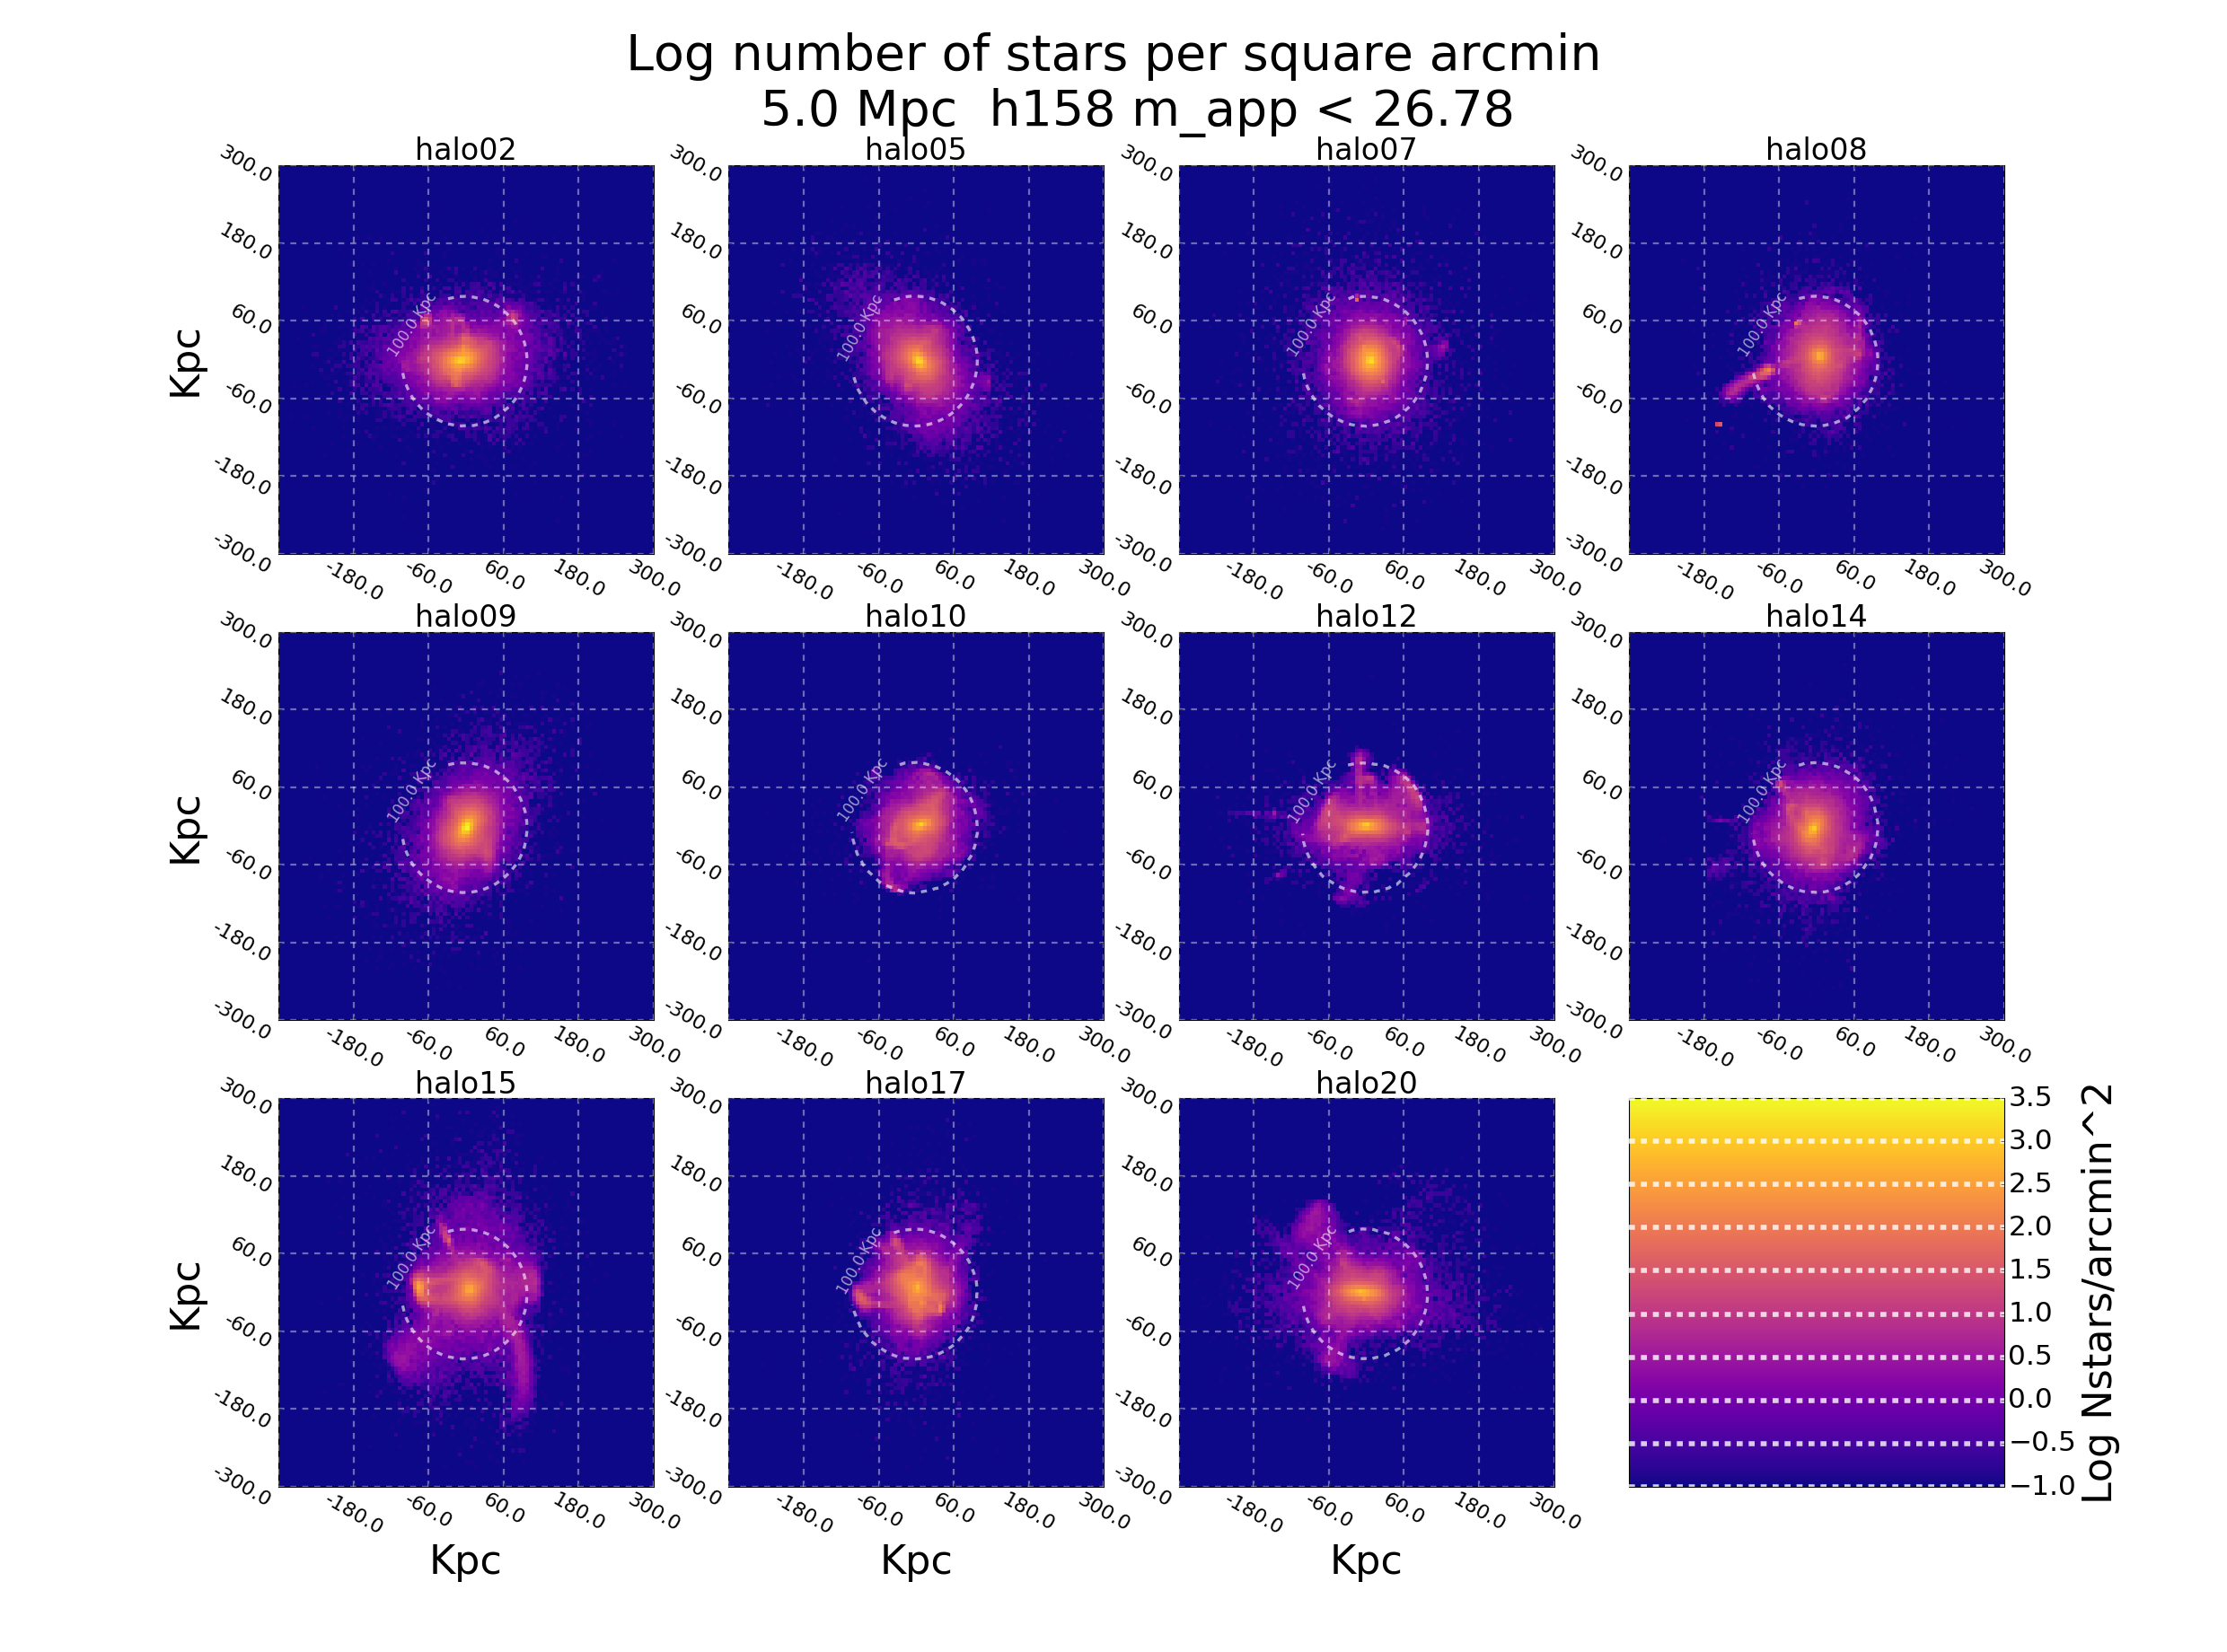
\includegraphics[width=17cm]{nstars_5Mpc_h158.png}
		\caption{
			Here we see the stars visible at 5 Mpc for all 11 halos projected and binned into a 100 x 100 grid.
			The grid covers a halo area of 600 x 600 Kpc.
			A 600 Kpc box has a radial separation of 300 Kpc.
			Halo stars are rendered at 5 Mpc using WFIRST filter h158.
			We can see that star counts $>$\ 25 per square arcmin out to separations of 100 to 150 Kpc.
			5 Mpc distance is chosen because the mean target distance from our 100 targets is 4.54 Mpc.
			The white circle indicates a radial separation of 100 Kpc.
		}
		\label{fig:log Nstars per sqdeg}
		\end{figure}
	% subsection broad_expectations (end)

	\subsection{Understanding the data} % (fold)
		\label{sub:understanding_the_data}
		Regarding our choice of magnitude limit at 26.78 we have taken the following factors into account.
		First there are the limits of the WFIRST filters and second there are the limits presented by star galaxy separation. 
		To adjust the known WFIRST filter limits $(imaging\ depth)$\ we are currently using the best information available to us by word of mouth and the recent findings of P.Madau \& L. Pozzetti $(N_{galaxies}\ area^{-1}\ 0.5\ mag^{-1})$.
		For now the assumption is that we will be able to separate our targeted halo stars from distant background galaxies within 1 magnitude of any given WFIRST filter limit $(imaging\ depth)$.

		The following plots show us the log value of the number of halo stars with $m_{app}<26.78$\ per $arcmin^{2}$\ ($Log(Nstars)/arcmin^{2}$).
		These are the stars apparently brighter than 1 magnitude less than WFIRST filter H158's 2000 second apparent magnitude limit ($m^{H158}_{2000sec}limit-1=26.87$).
		%We also plot the $Log(N_{galaxies})/arcmin^{2}$\ determined by Madau \& Pozzetti for $m_{app}$\ 26.87 as a horizontal line.
		Compared to the previous plots these are paired with a scatter plot of radial separation (x-axis) and $Log(Nstars)/arcmin^{2}$\ (y-axis) for a $(600\ Kpc\ box)$\ and a zoom in showing a 360 Kpc box.
		Each point on the scatter plot represents one of the 10,000 bins from the grid displayed in the center column.
		The third column is a zoom in of the second column.
		Stars within the area between the white circles correspond to the orange points on the scatter plot.

		These plots show that at a distance of 2 Mpc we will safely have star counts $>$ 100 per $arcmin^{2}$\ at separations from 100 to 150 Kpc.
		At 5 Mpc, however, the counts drop as low as 10 stars per $arcmin^{2}$.
		Discussion point: star-galaxy limits? 
		\begin{figure}[H]\centering
			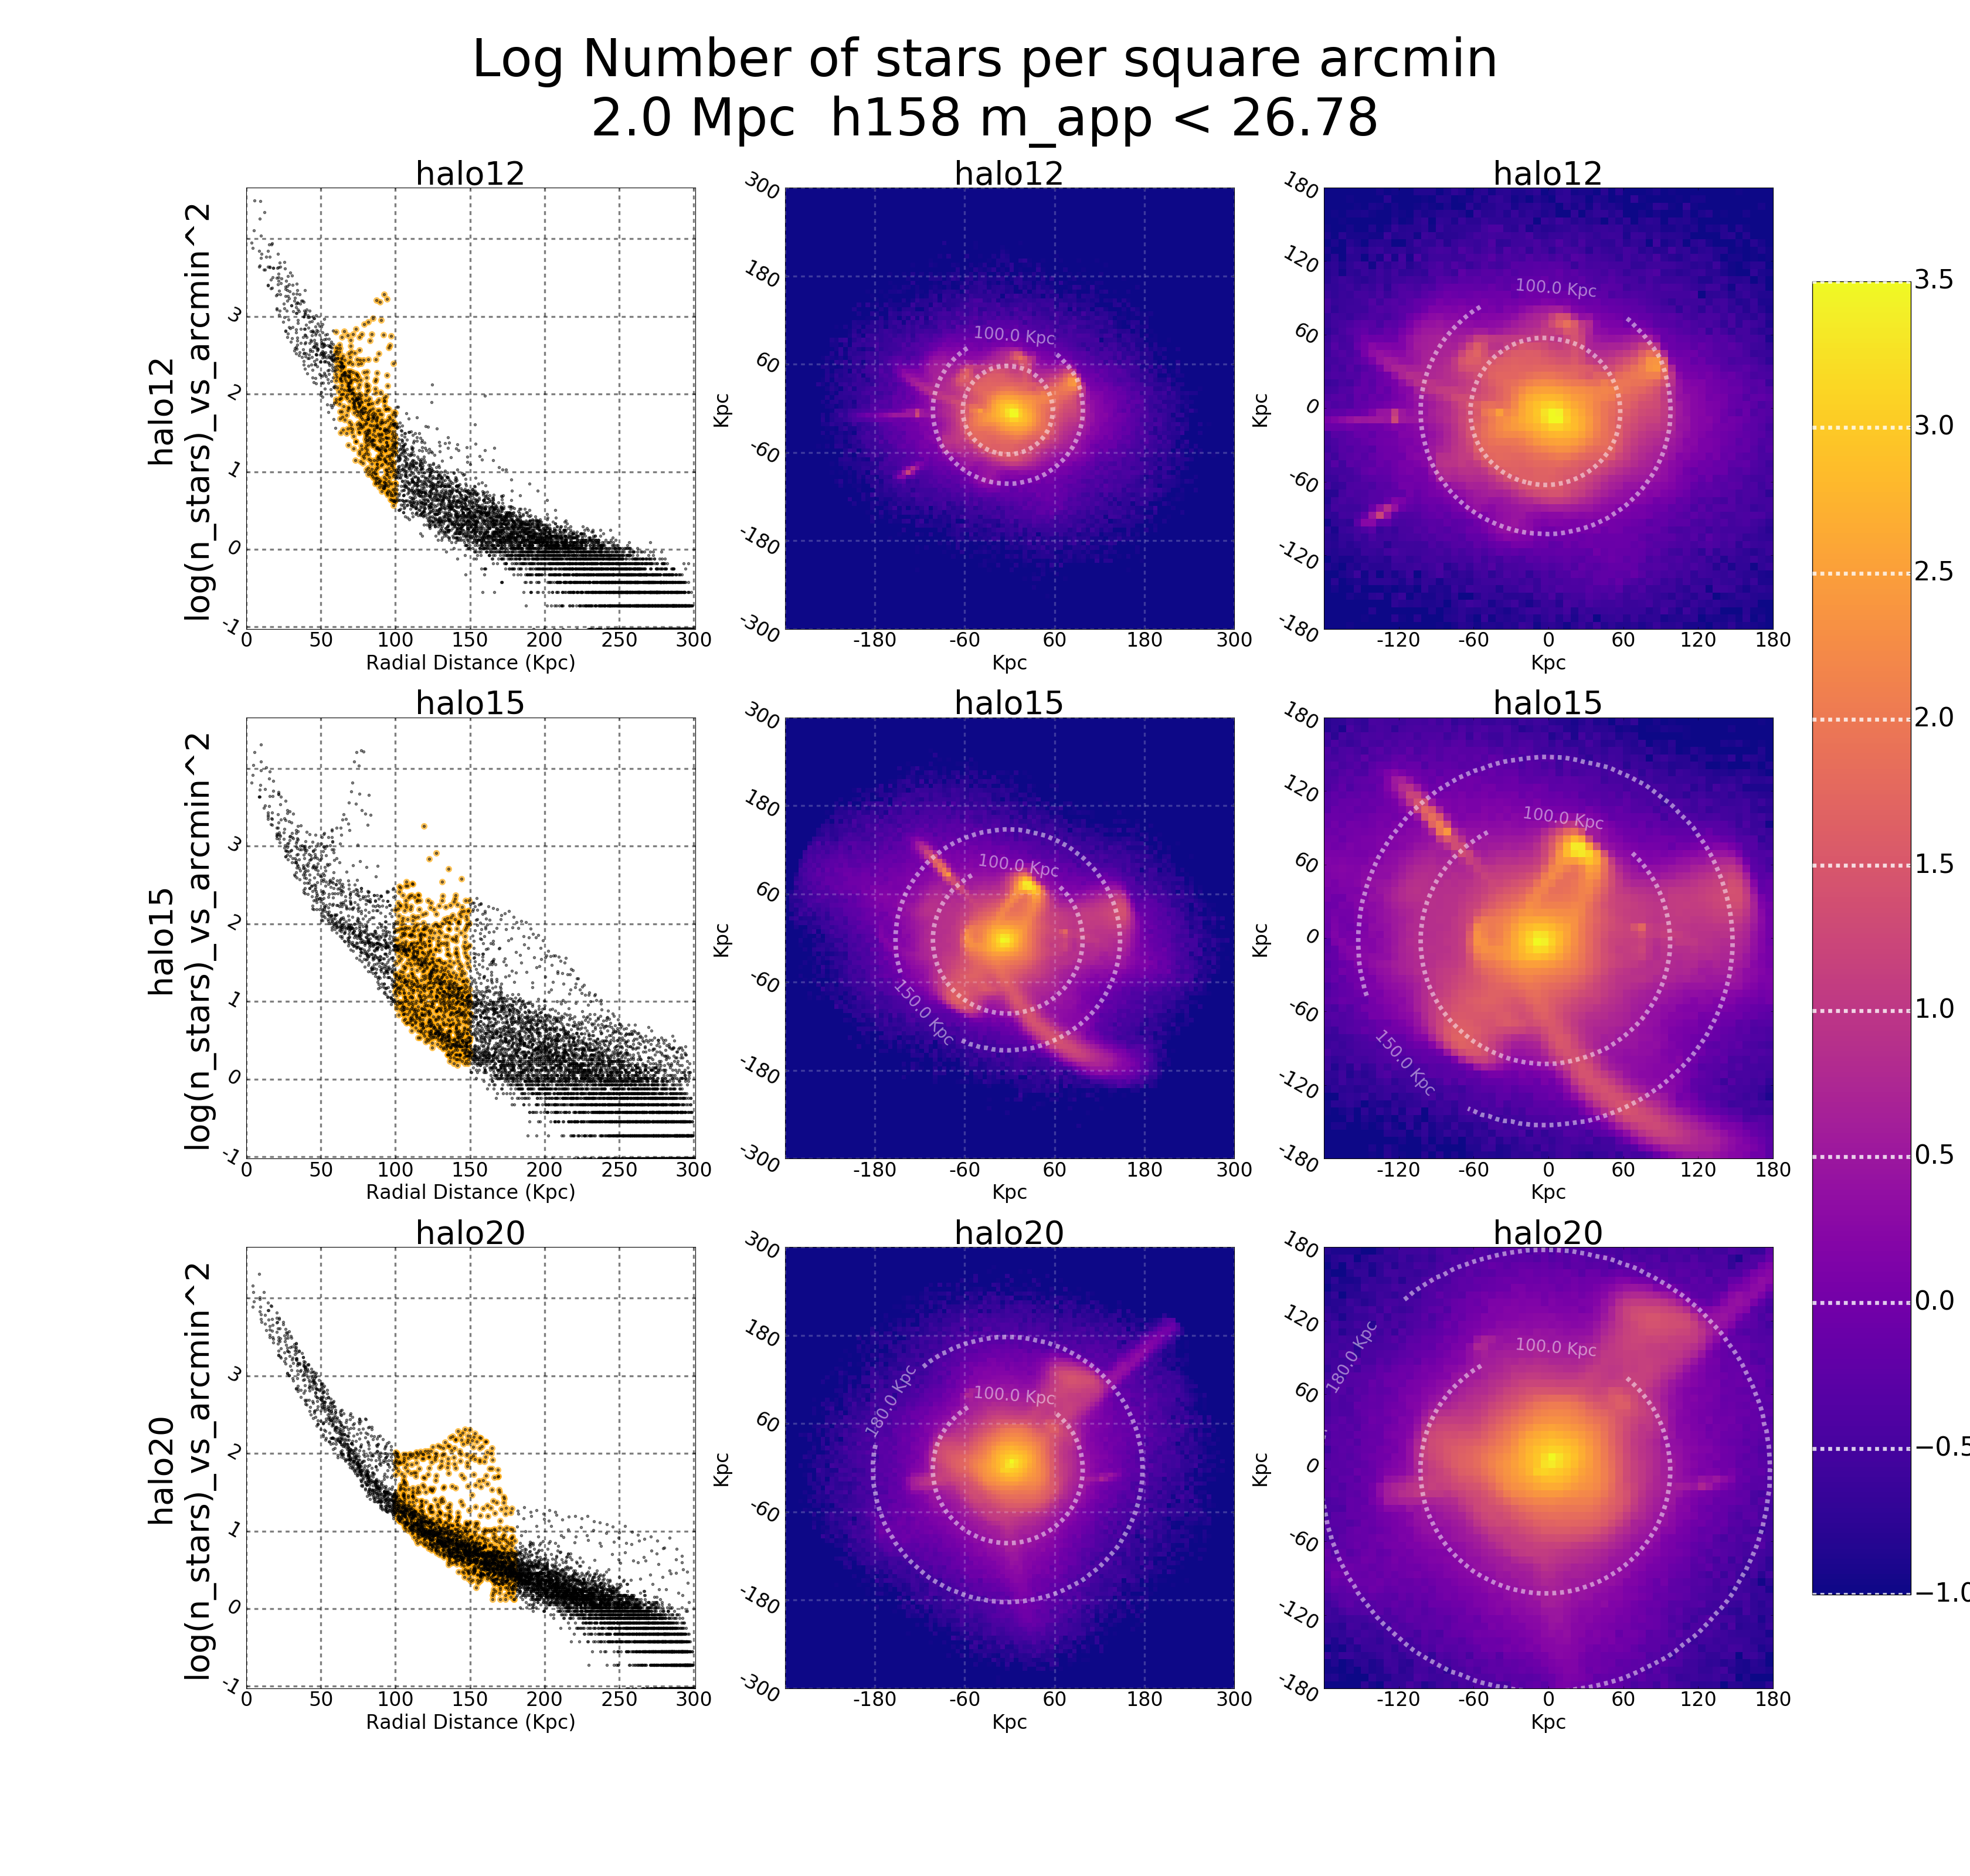
\includegraphics[width=17cm]{mixplt_2Mpc_h158.png}
		\caption{
			Here we see halos 12, 15 and 20 displayed at $2\ Mpc$\ and viewed with WFIRST filter $H158$.
			The first column shows a scatter plot with x-axis representing $0\ to\ 300\ Kpc$\ projected radius (600 Kpc box) vs y-axis the log10 number of stars per square arcmin with $m_{app}<26.78$.
			The second column shows the same log value out to a radius of 300 Kpc (600 Kpc box) as in figure 2.
			The third column shows a zoom in of the second column to a radius of 180 Kpc (360 Kpc box).
			Stars within the area between the white circles correspond to the orange points on the scatter plot.
		}
		\label{fig:mean_starclass_at_r_2Mpc}
		\end{figure}

		\begin{figure}[H]\centering
			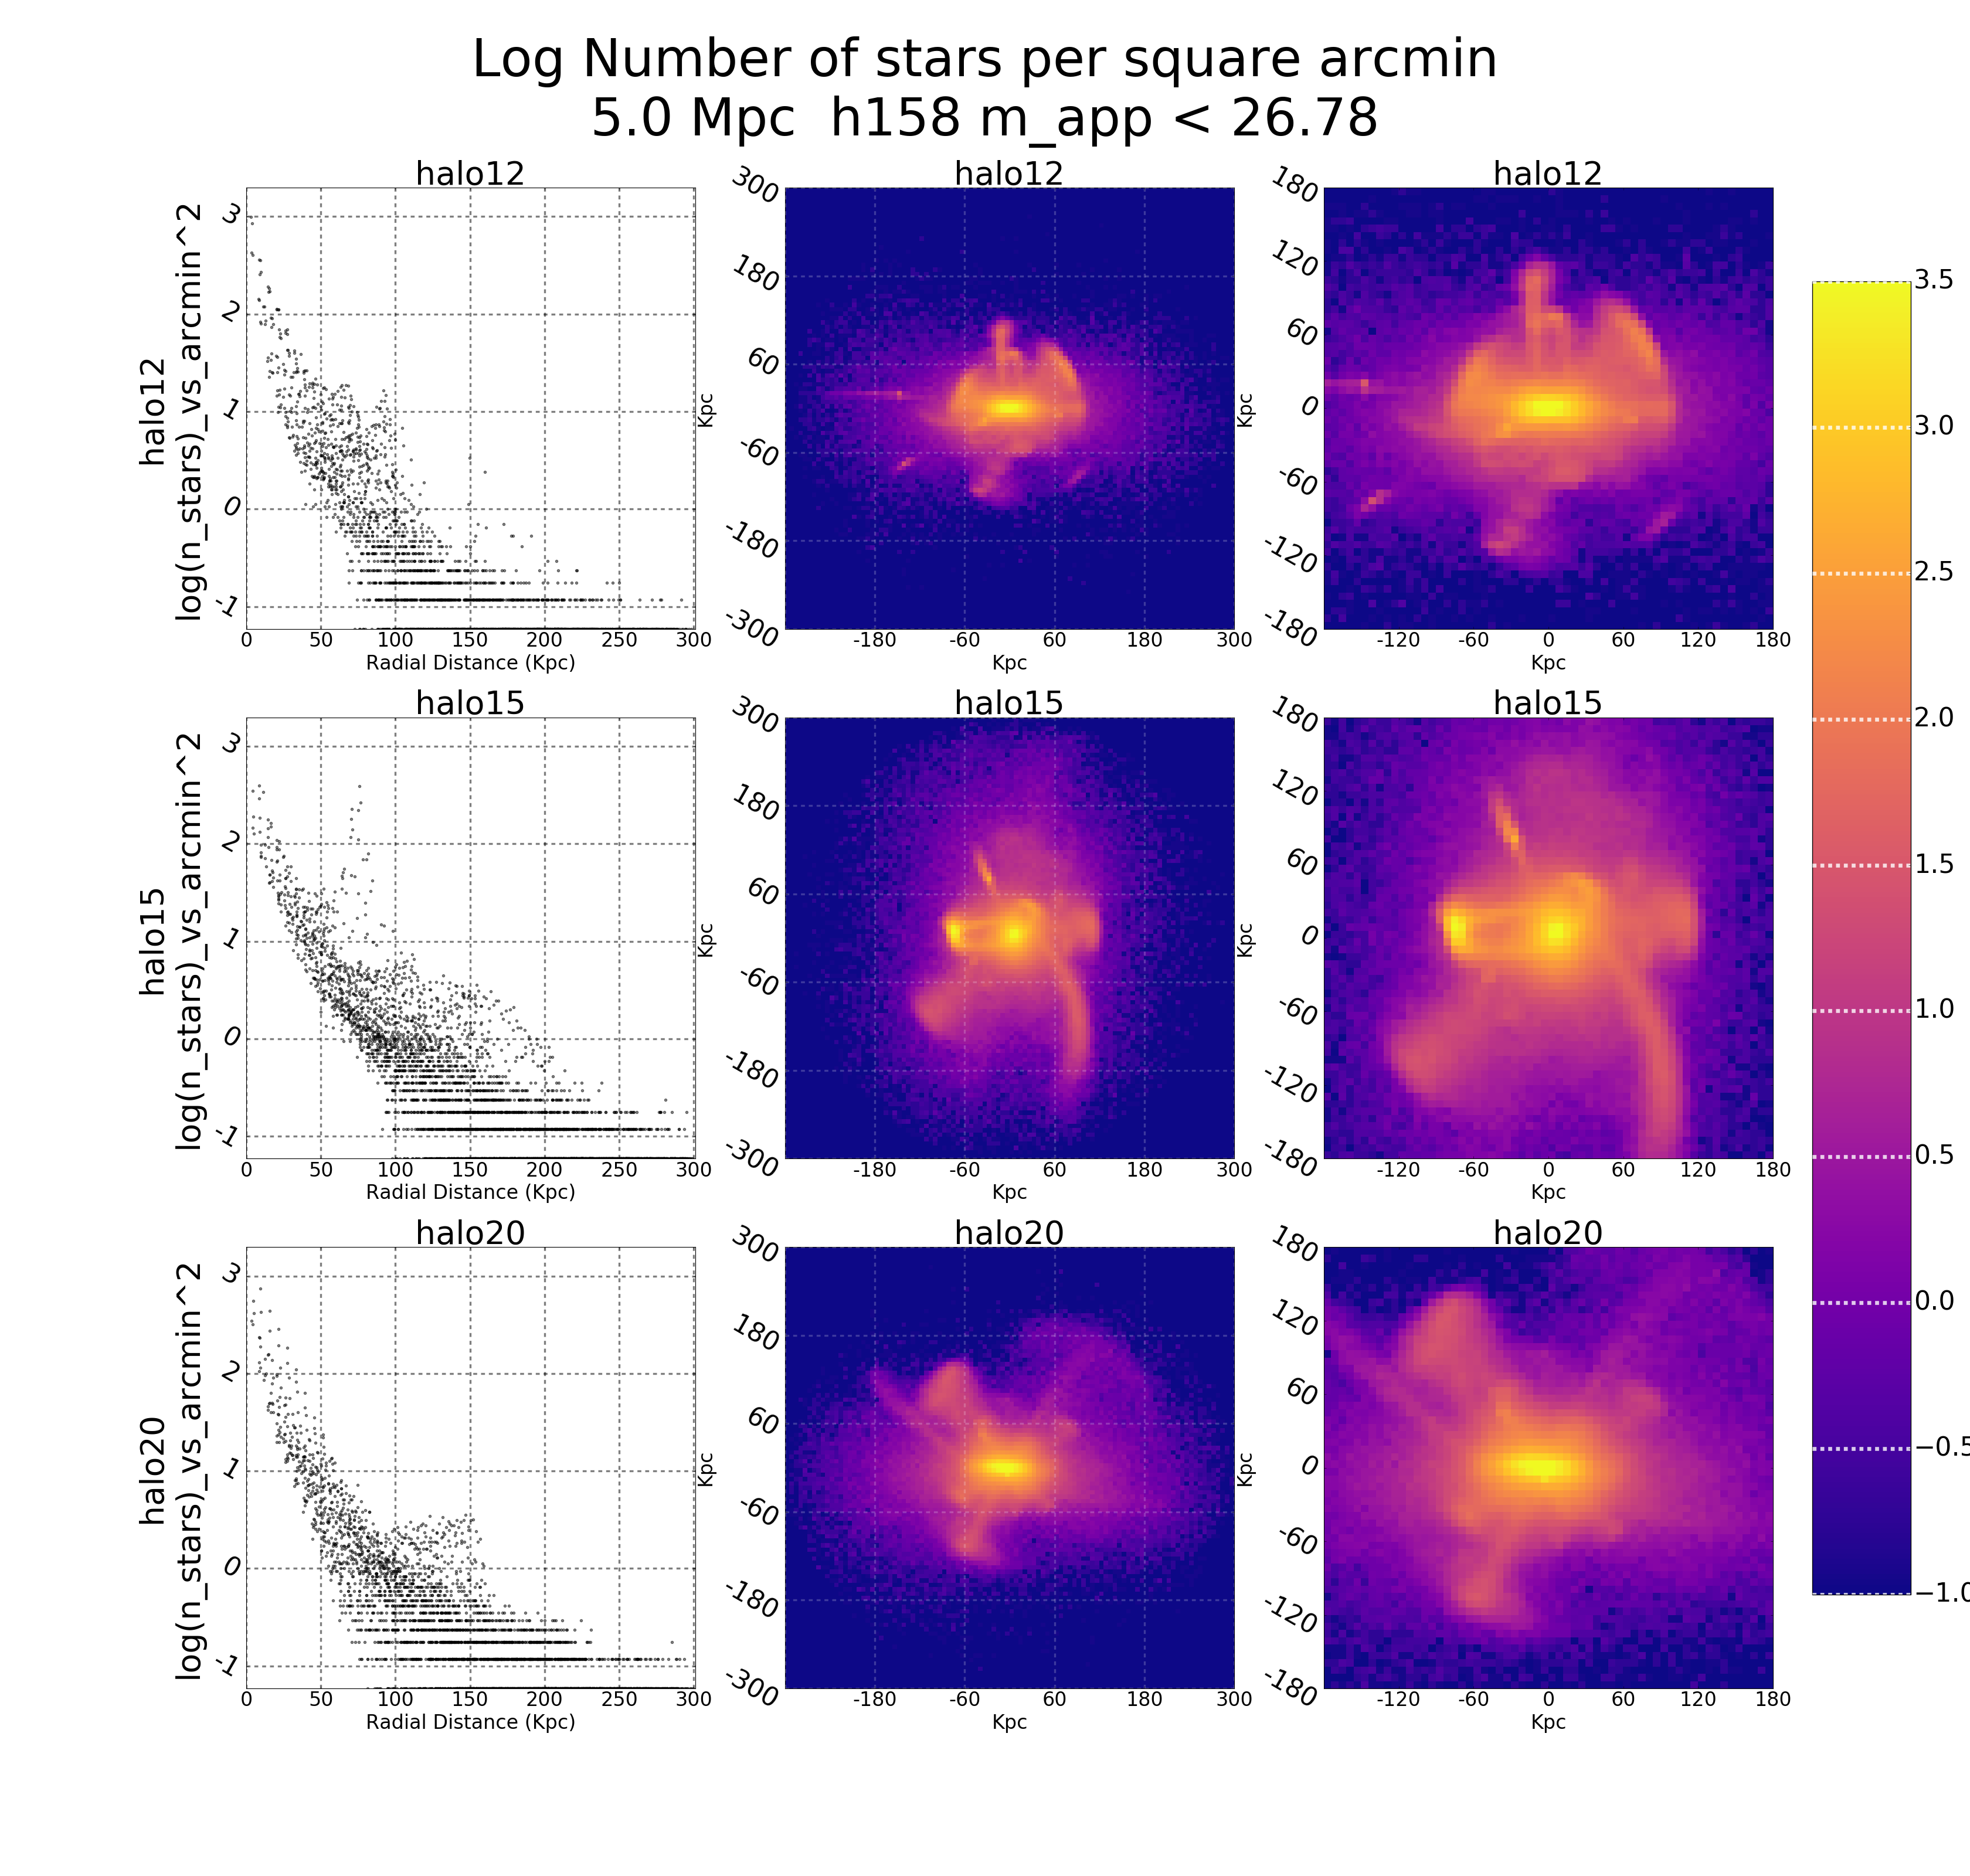
\includegraphics[width=17cm]{mixplt_5Mpc_h158.png}
		\caption{
			Again we see the same halos as in figure 3 but this time displayed at $5\ Mpc$.
		}
		\label{fig:mean_starclass_at_r_5Mpc}
		\end{figure}
	% subsection understanding_the_data (end)

	\subsection{Summary of all 11 Halos} % (fold)
		\label{sub:summary_of_all_11_halos}
		Bellow is figure 5, another scatter plot of the 10,000 bins from figure 2.
		Figures 5 and 6 show the log number of stars per square arcmin with $m_{app}<26.78$\ as a function of radius for all 11 halos.
		Figure 5 shows 2 Mpc and figure 6 shows 5 Mpc.

		\begin{figure}[H]\centering
			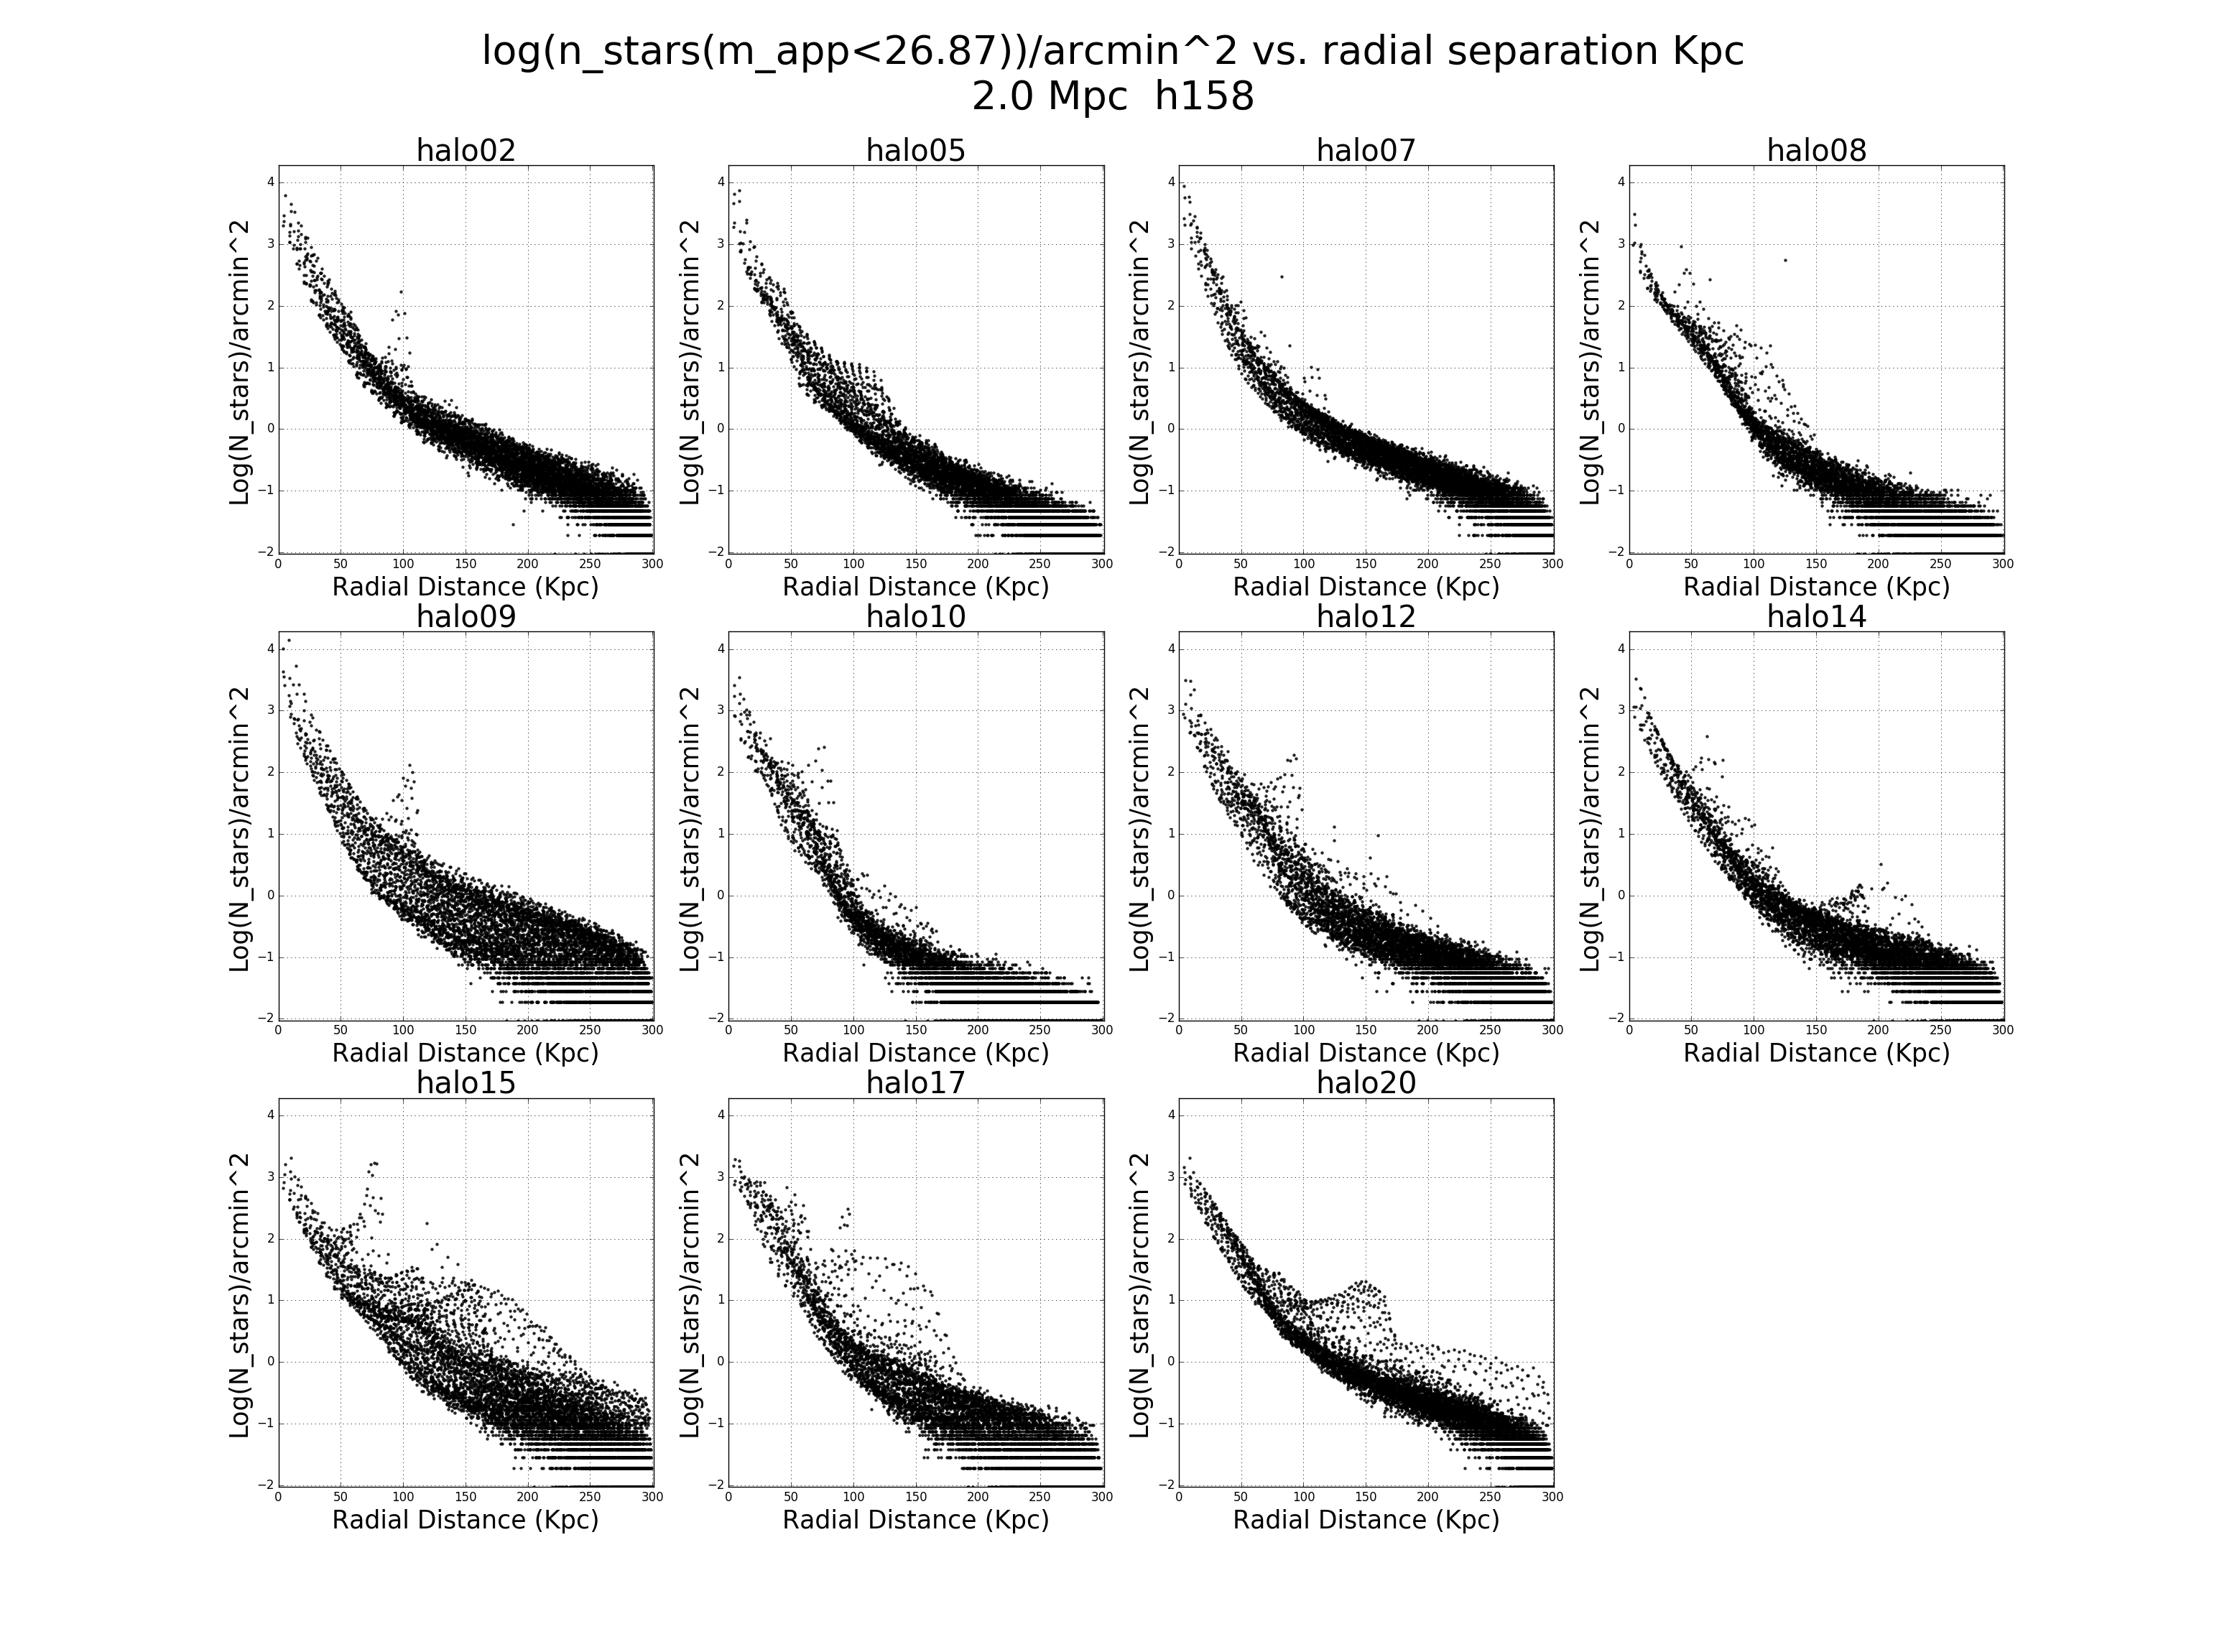
\includegraphics[width=17cm]{sqdeg_2Mpc_h158.png}
		\caption{
			Here we see each section of the 100 x 100 grid from figures 2.
			We have plotted the log number of stars ($m_{app}<26.78$)\ in each bin as a function of radius (Kpc).
			This plot is calculated ad 2 Mpc with WFIRST filter H158.
		}
		\label{fig:nstars as function of radius 2Mpc}
		\end{figure}

		\begin{figure}[H]\centering
			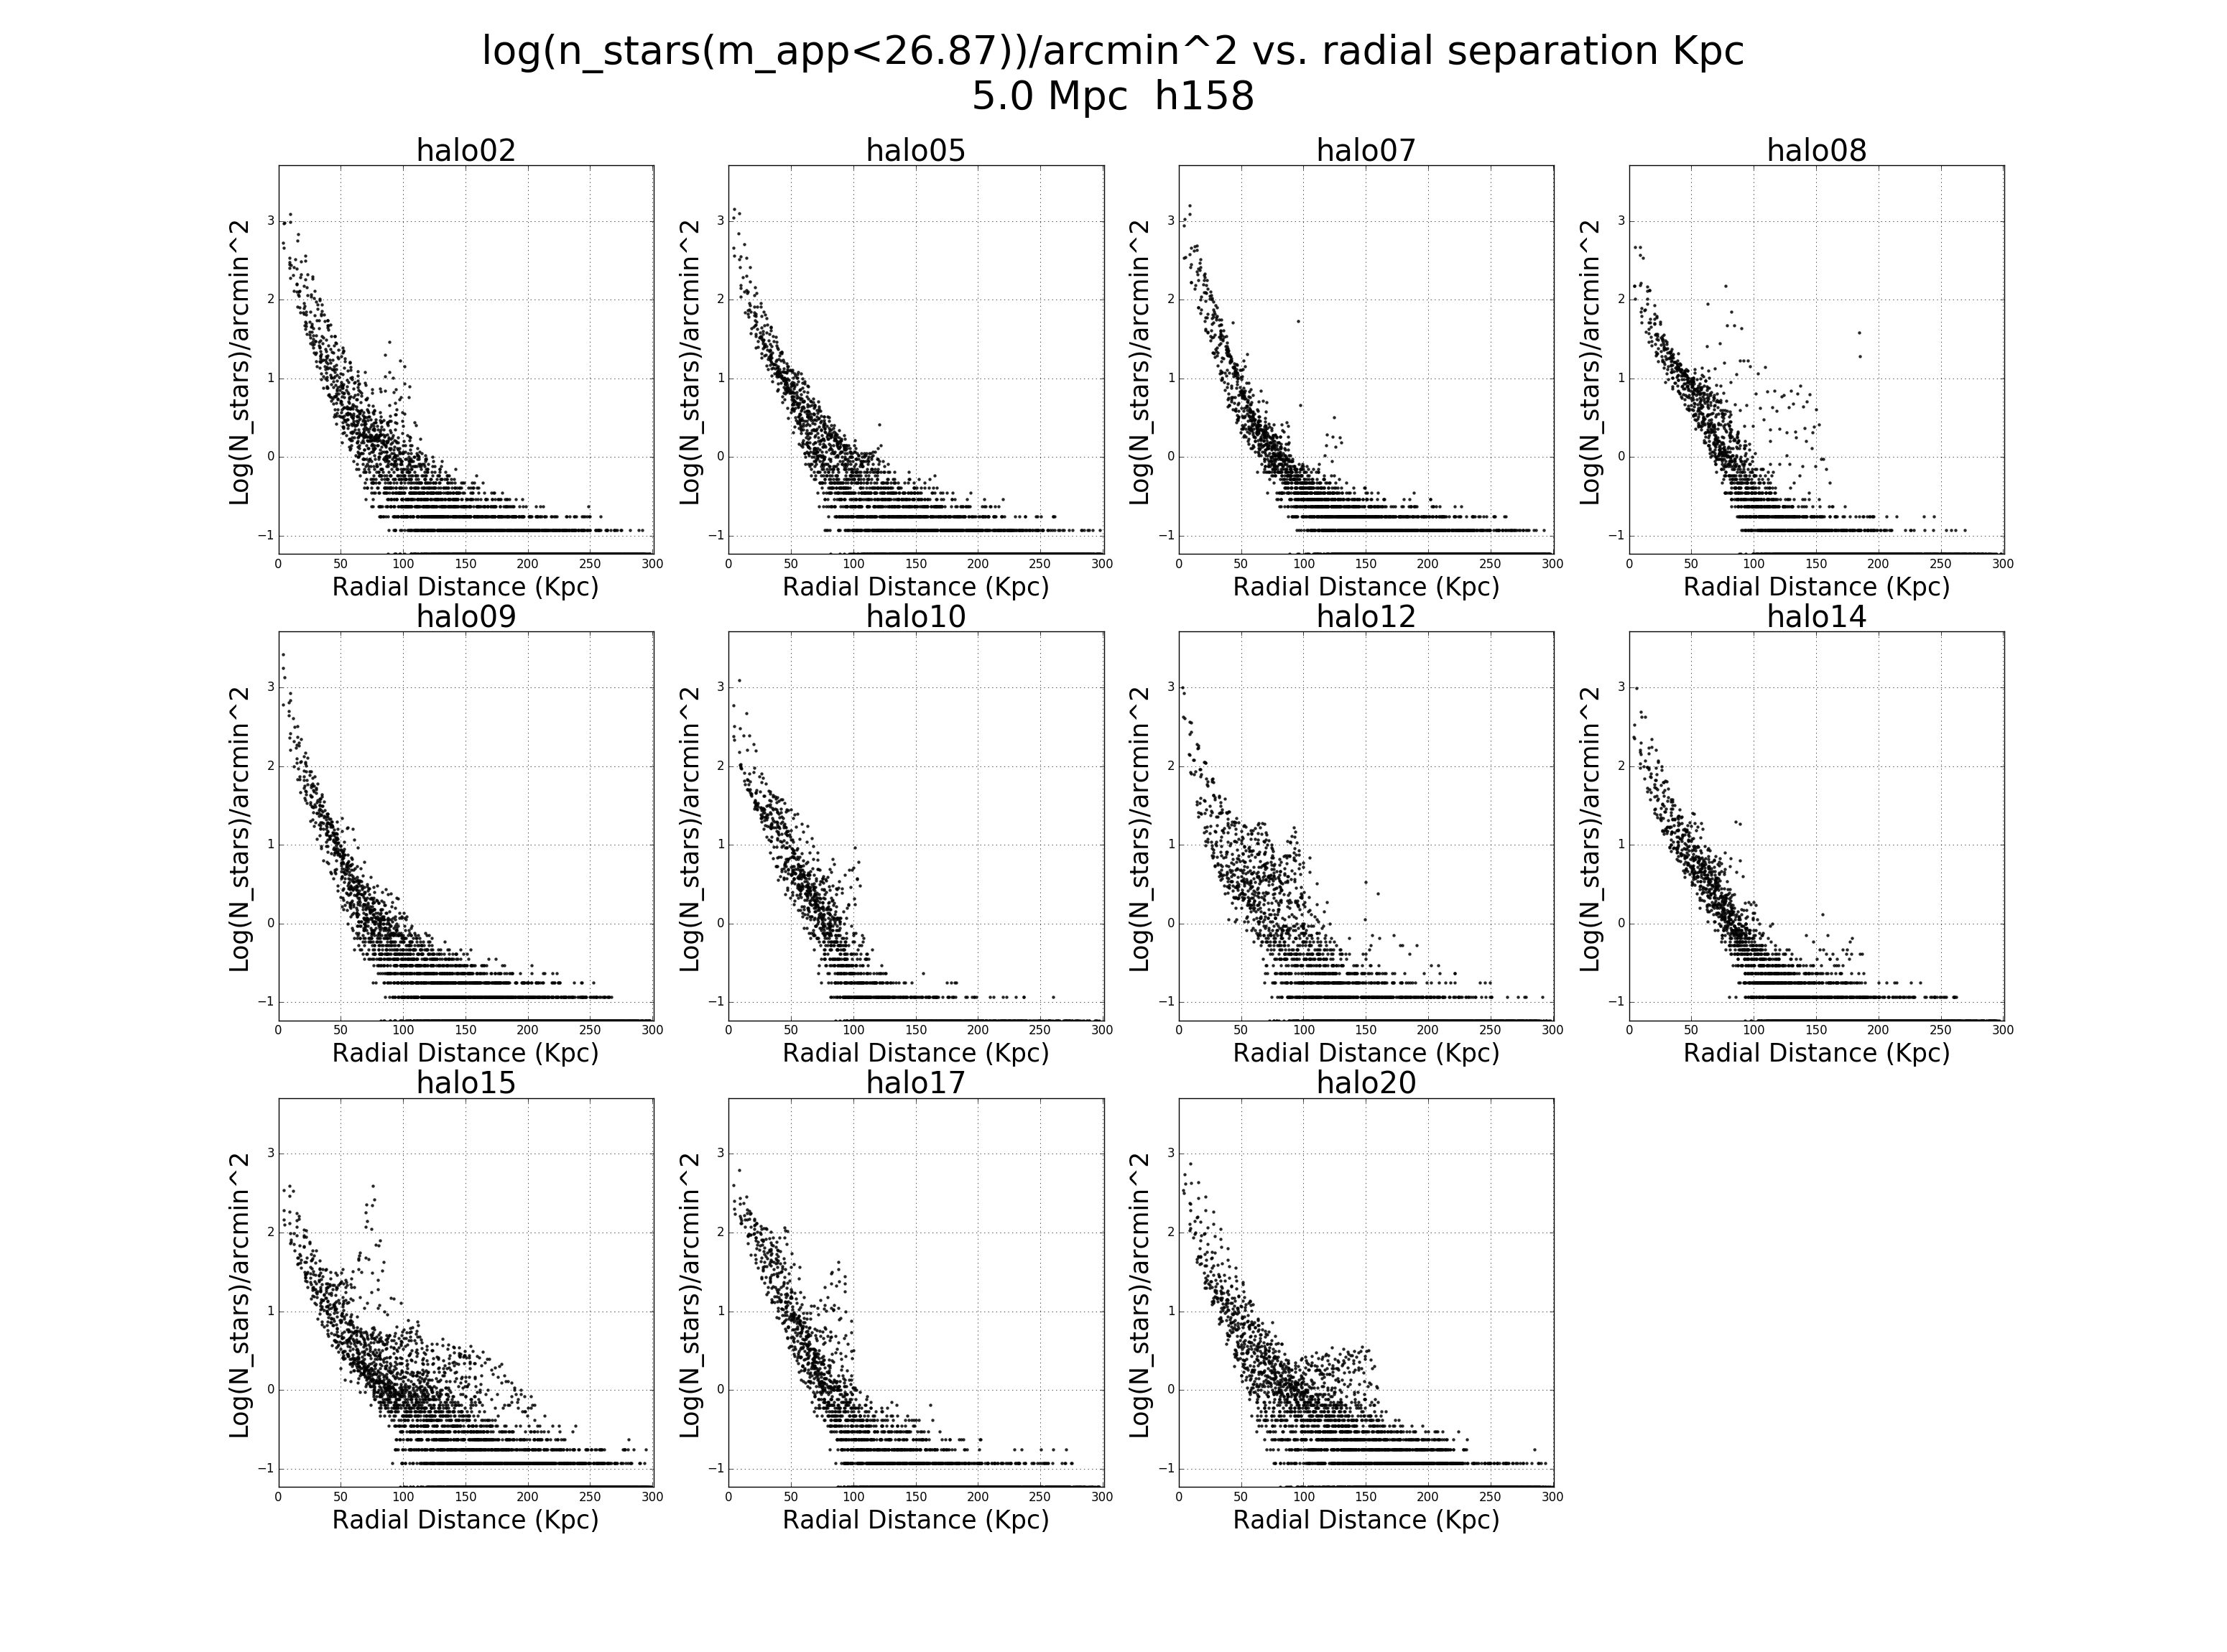
\includegraphics[width=17cm]{sqdeg_5Mpc_h158.png}
		\caption{
			Once again we see the same plot as in figure 5 but this time rendered at an estimated distance of 5 Mpc instead of 2 Mpc.
			2000 second exposure and WFIRST filter H158.
		}
		\label{fig:nstars as function of radius 5Mpc}
		\end{figure}

		Bellow is figure 7.
		Figure 7 consists of three color and apparent magnitude diagrams (2, 5, 8 Mpc) for all halo stars belonging to Johnston/Bullock halo02.
		We can see the same three lines representing the P.Madau \& L. Pozzetti magnitude limits and log number of galaxies per square arcmin.

		\begin{figure}[H]\centering
			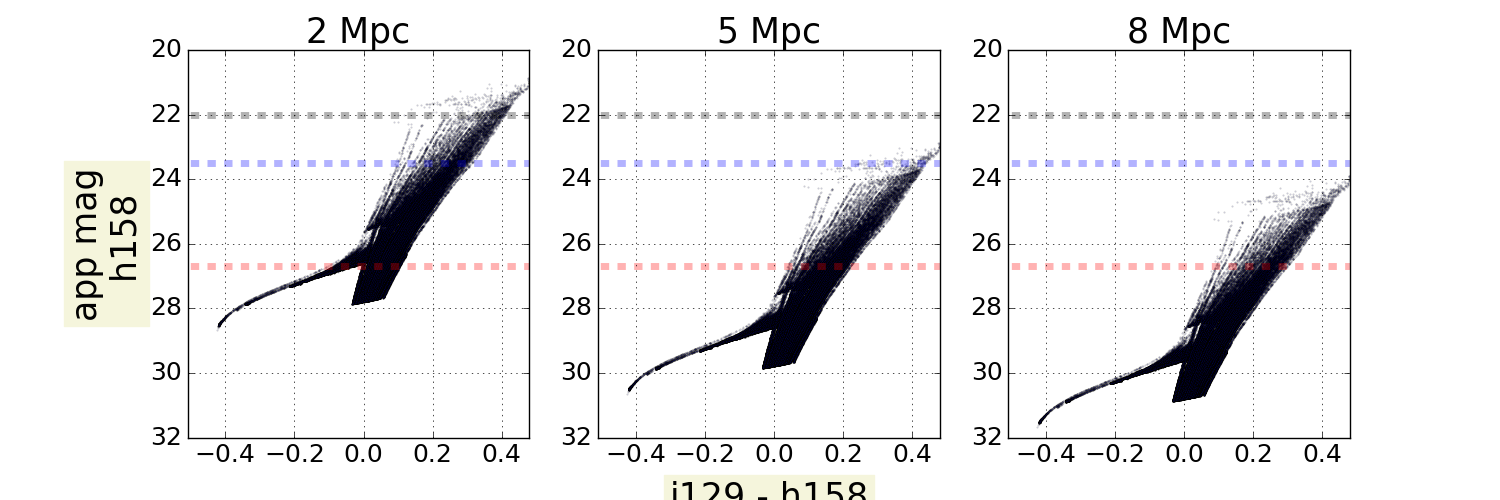
\includegraphics[width=17cm]{cmd.png}
		\caption{
			This is a cmd for apparent magnitude in WFIRST filter h158 and color for WFIRST filters $($j129 $-$\ h158w$)$\ rendered at distances of 2, 5, 8 Mpc.
			The max distance of our 100 targets is 7.2 Mpc.
		}
		\label{fig:cmd}
		\end{figure}
	% subsection summary_of_all_11_halos (end)
% section interpreting_simulated_data (end)

\section{Looking forward:} % (fold)
	\label{sec:looking_forward}

	$1.$\ Star-galaxy separation limits.\\

	$2.$\ Different simulated data sets in addition to 11 Bullock/Johnston stellar halo models.\\

	$3.$\ Better definitions for halo features and observational limits thereof.\\
% section looking_forward (end)

%% --------------------------------------------------------------------------
%% BIBLIOGRAPHY
%% --------------------------------------------------------------------------
\bibliography{mylib}{}
\bibliographystyle{plain}

%% --------------------------------------------------------------------------
%% END DOCUMENT
%% --------------------------------------------------------------------------
\end{document}



